\documentclass{article}
\usepackage{sidecap}
\usepackage{color}
\usepackage{graphicx}
\usepackage{amsmath}
\usepackage{mathtools}
\usepackage[paperwidth=28in,margin=0.5in]{geometry}
\begin{document}
\begin{SCfigure}
\caption{From the URAT1 database we collected data on about 1 million stars in the from the area around the center of the cluster.  All of these stars fell within the observed tidal radius of the cluster.  Using our collection of candidate stars we measured the average density of stars per square degree on the plane of the sky.  We calculated that about 700 more stars were found in this area, than the average predicted.  This implies that around 300 more stars should be added to our set of previously identified members.  All other thing unkown this could be the estimate of whether a star is a member or not. $p(M)$

We found the mean location, and of the proper motions of the known members of the cluster. We calculated the distance from these center point for each star in the cluster.  Using the distances of the member stars we fit a probability distribution.  This distribution was a measure of the probability density of having a particular distance from he center if one assumed that a star was a member $p(R|M)$, in either geometric space or proper motion space respectively.  

We combined the set of identified members, and other stars in the are, and used these to fit other probability density functions.  We treated these as the probability of a star having a particular radial distance. $p(R)$ 

Using Bayes's theorem for conditional probability we calculated the probability of a star being a member given the radial distance. $P(M|R)$. Bayes's theorem states:
\begin{equation}
P(A|B)=\frac{P(B|A)P(M)}{P(A)}
\end{equation}
Using these we calculated the probabilty of each star being a member given their radial distance in both proper motion and geometric space}
\begin{subfigure}{0.5\textwidth}[tr]{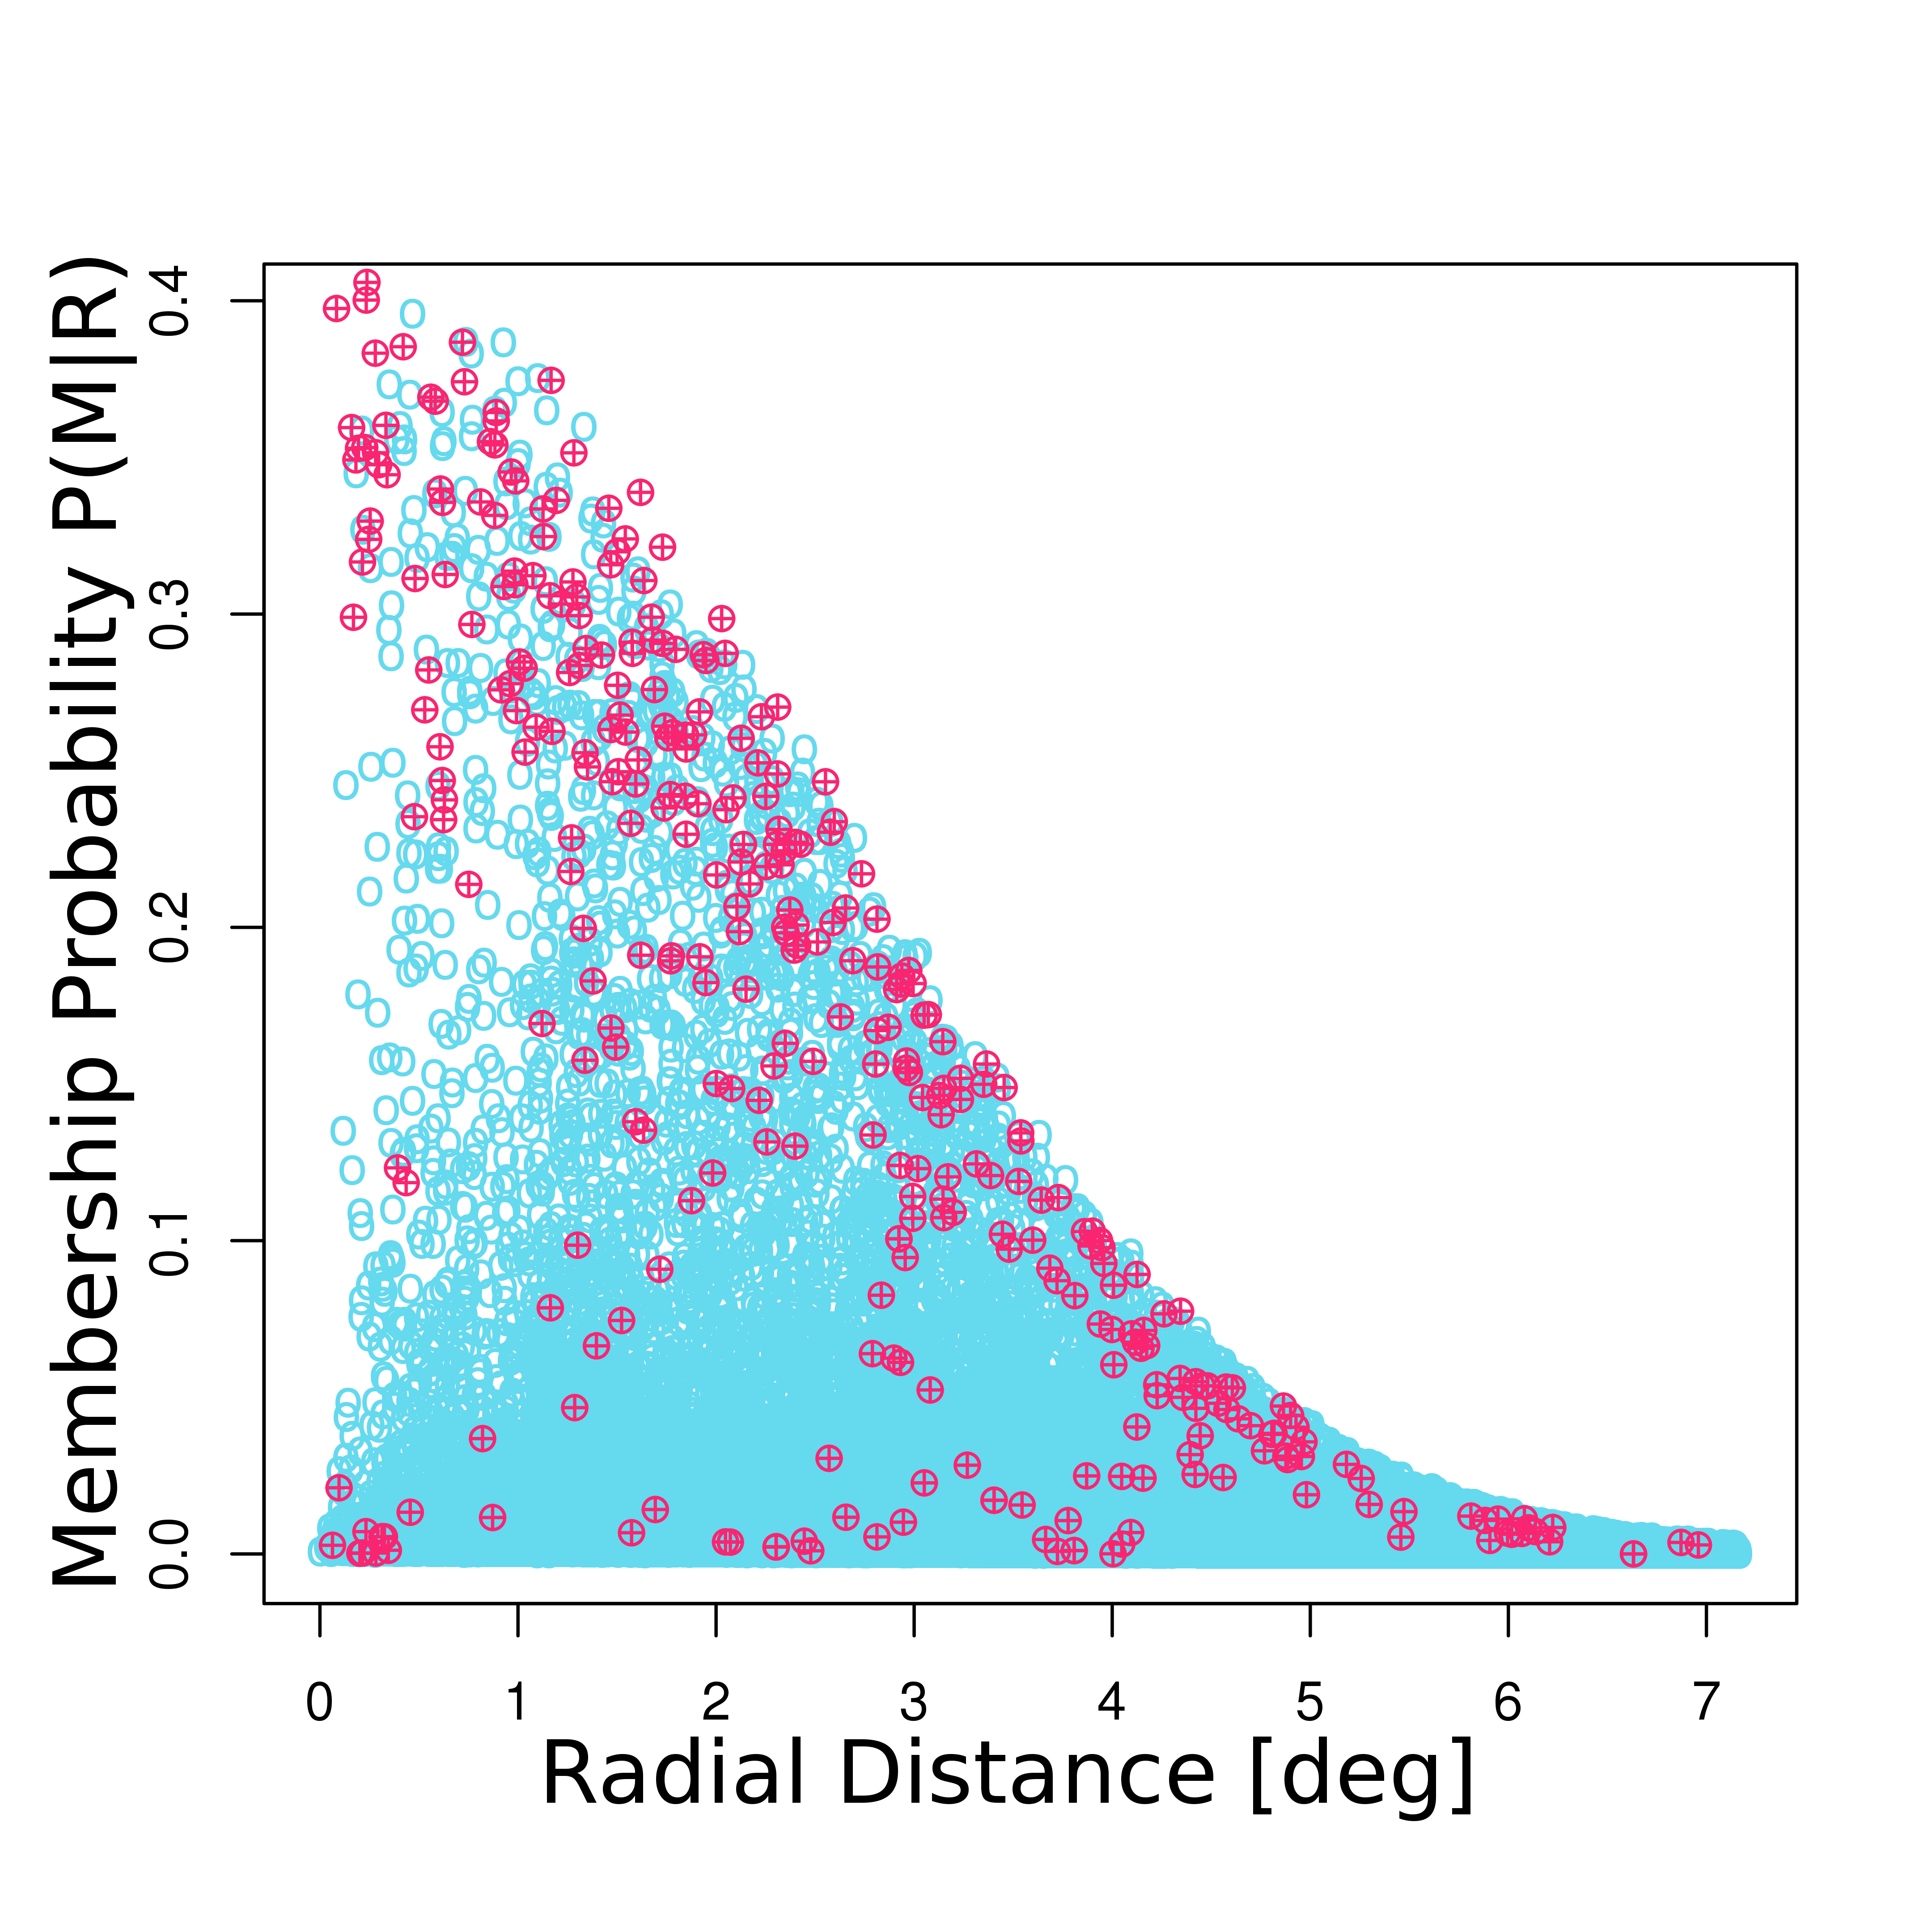
\includegraphics{SpaPro}}
\end{subfigure}
\begin{subfigure}{0.5\textwidth}[tr]{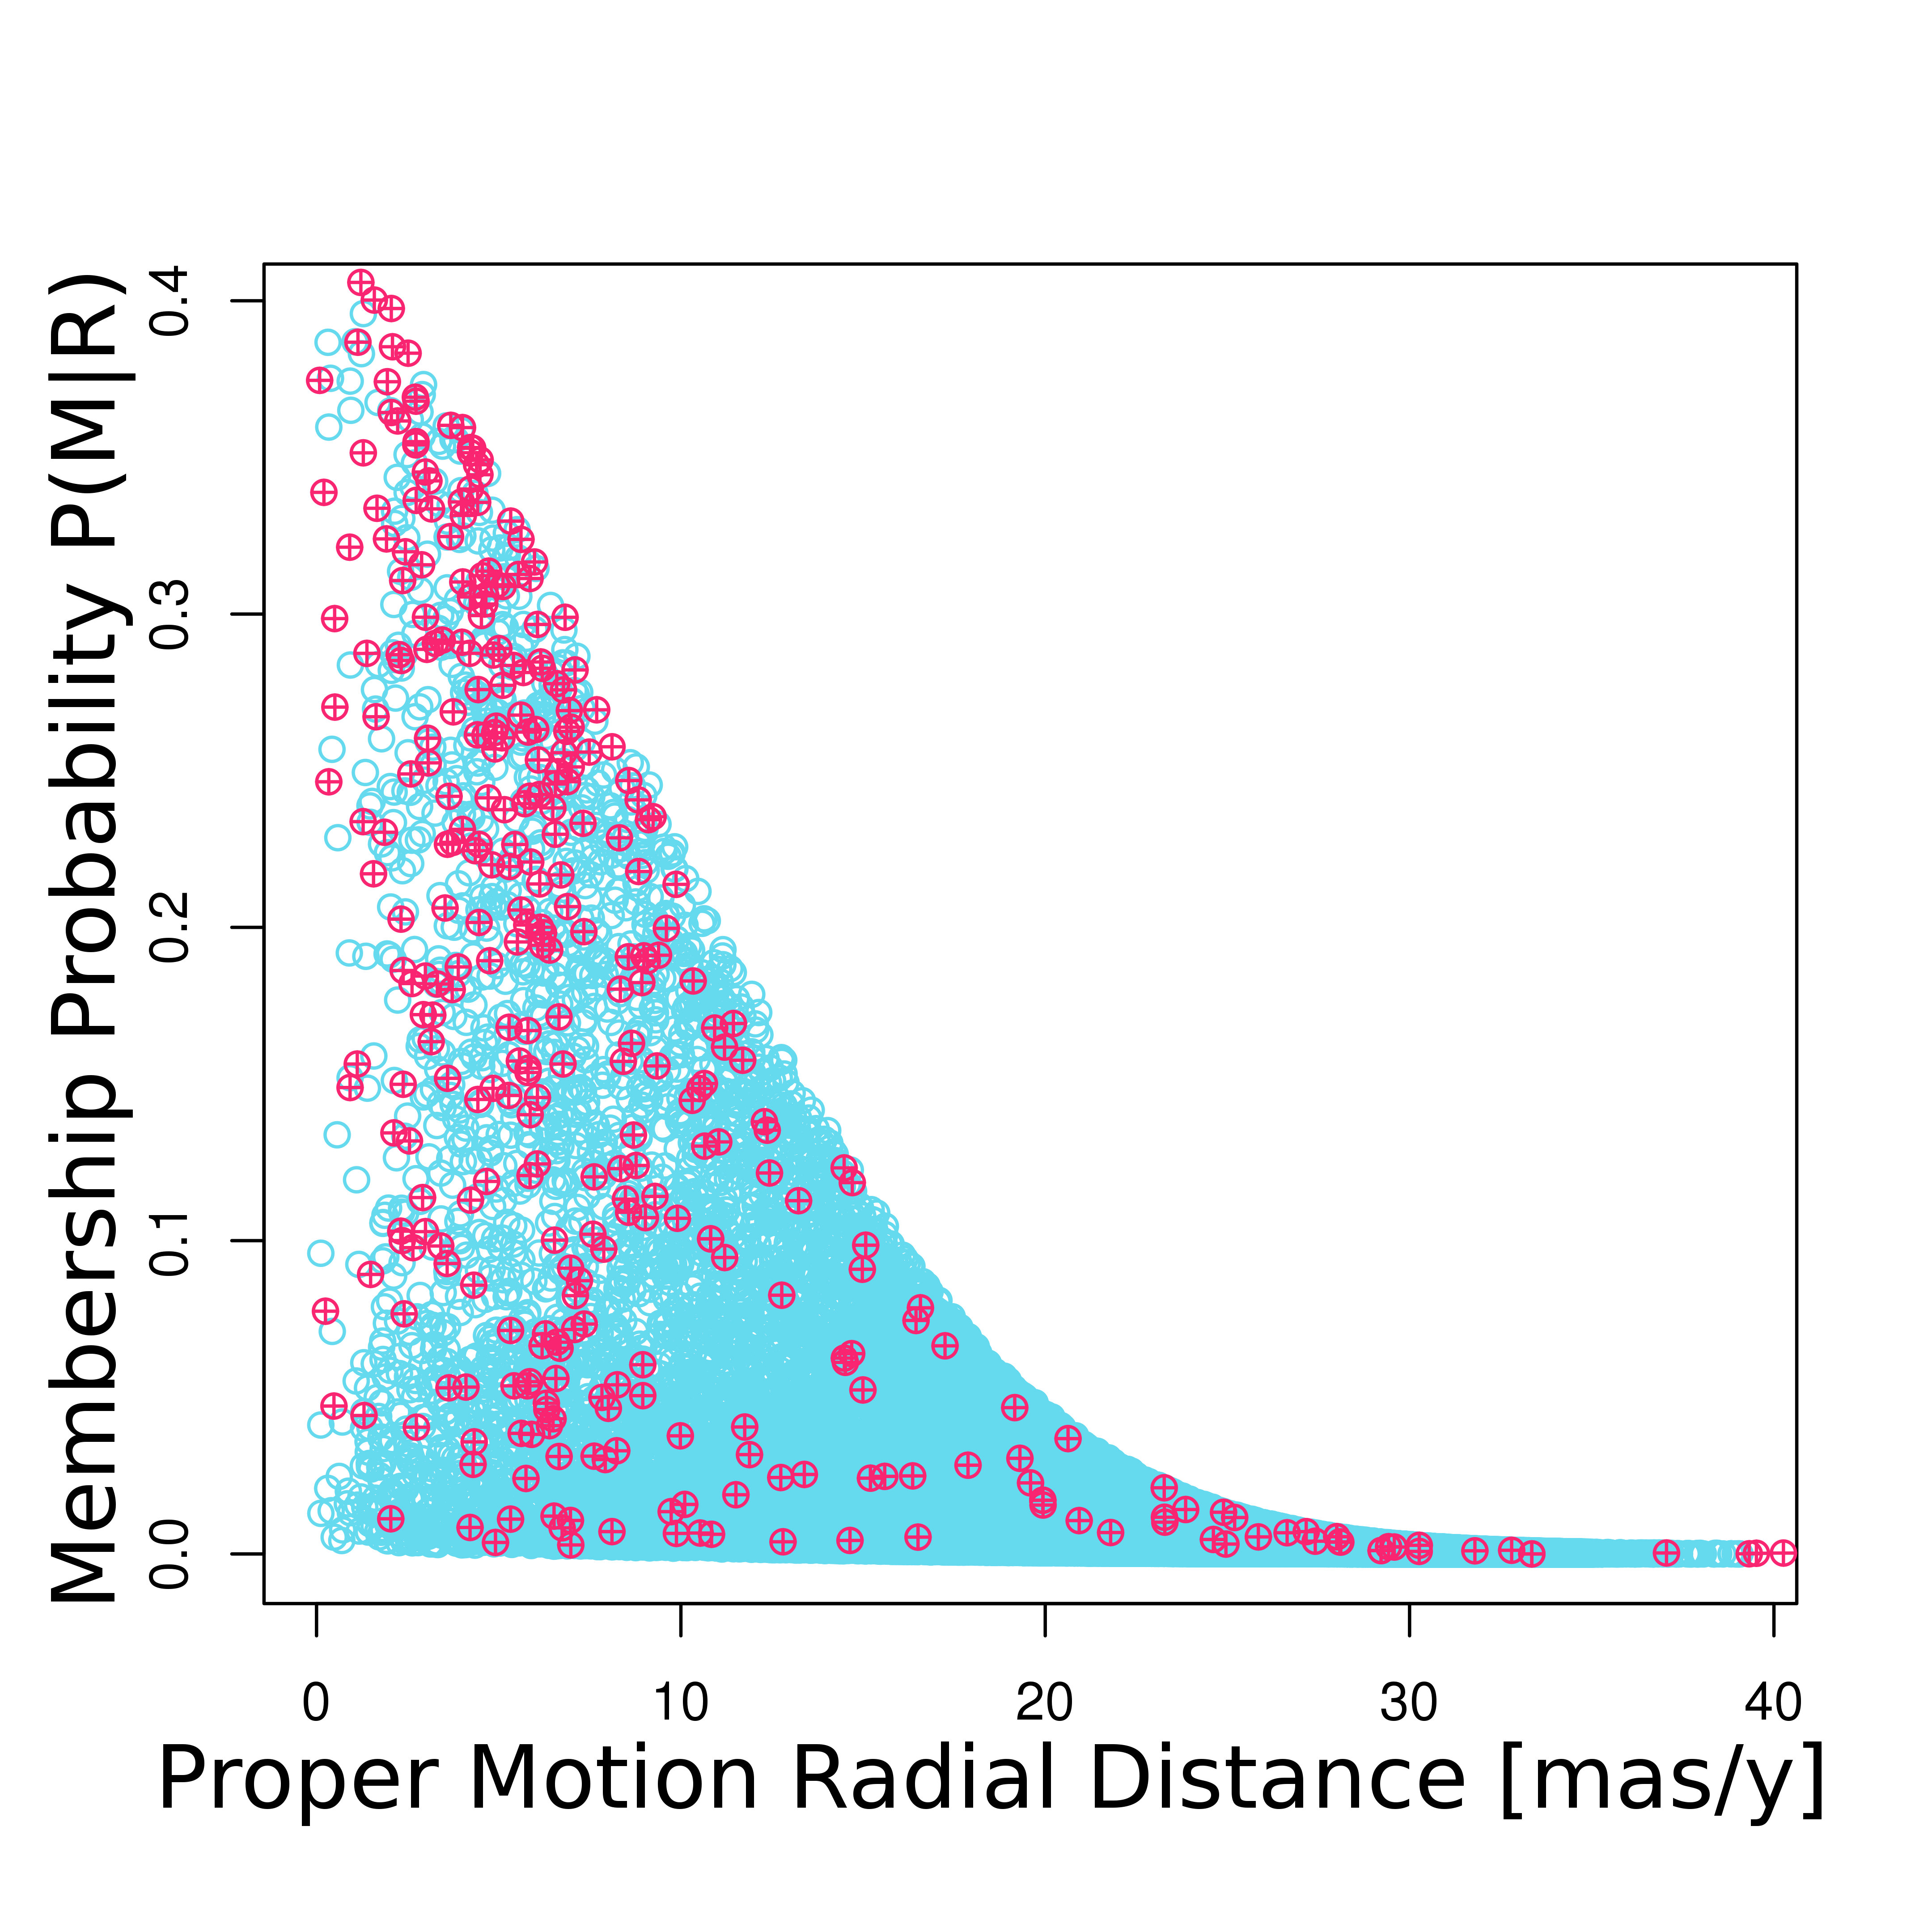
\includegraphics{ProPro}}
\end{subfigure}
\end{figure}
